\documentclass[11pt]{report}

\usepackage[utf8]{inputenc}
\usepackage[T1]{fontenc}
\usepackage[french]{babel}
\usepackage{amsmath}
\usepackage{amssymb}
\usepackage{graphicx}

\usepackage{listings}
\usepackage[dvipsnames]{xcolor}

\lstdefinelanguage{pdl}{
  keywords={Si, ALORS, Sinon, finSi, Pour, allant de,  FAIRE, finPour, tantQue, finTantQue, fonction, finFonction, action, finAction, Struct, finStruct, dansLeCasDe, case, default},
  keywordstyle=\color{RedOrange}\bfseries,
  keywords=[2]{booleen, chaine, entier, reel, caractere},
  keywordstyle=[2]\color{NavyBlue}\bfseries,
  keywords=[3]{retourner, constante},
  keywordstyle=[3]\color{Plum}\bfseries,
  identifierstyle=\color{black},
  sensitive=false,
  comment=[l]{//},
  morecomment=[s]{/*}{*/},
  commentstyle=\color{Gray}\ttfamily,
  stringstyle=\color{ForestGreen}\ttfamily,
  morestring=[b]',
  morestring=[b]"
}

\lstset{
   language=pdl,
   extendedchars=true,
   basicstyle=\footnotesize\ttfamily,
   showstringspaces=false,
   showspaces=false,
   tabsize=3,
   breaklines=true,
   showtabs=false
}


\title{Analyse de jeu}
\author{Rachel \textsc{Humbert} \and Emma \textsc{Mange} \and Alphée \textsc{Grosdidier} \and Anton \textsc{Dolard} \and Silvio \textsc{Vescovo}}
\date{\today}

\newcommand{\R}{\mathbb{R}}
\newcommand{\ex}{\stepcounter{Exercice} Exercice n°\arabic{Exercice} : }
\newcommand{\qu}{\stepcounter{Question} Question \arabic{Exercice}.\arabic{Question}. }
\newcommand{\lettre}{\stepcounter{Lettre} \alph{Lettre}) }

\makeatletter
\def\maketitle{
  \newpage
  \null
  \vskip 2em
  {\raggedright 
\includegraphics[scale=0.2]{nom_universite.png}\hspace{\stretch{1}}
\includegraphics[scale=0.4]{reseauFigure.png}}
  \begin{center}
  \let \footnote \thanks
    {\Huge \textbf{\@title} \par}
    \vskip 1.5em%
    {\large
      \lineskip .5em%
      \begin{tabular}[t]{c}
        \@author
      \end{tabular}\par}
    \vskip 1em%
    \vspace{\stretch{1}}
    \begin{minipage}{0.48\textwidth}
    {\large Puyo Puyo}
    \centering
    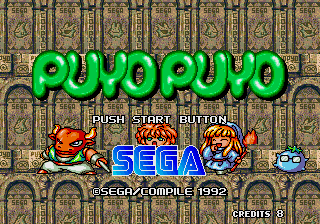
\includegraphics[width=\textwidth]{Puyoarc_e.png} 
	\end{minipage}
	\begin{minipage}{0.48\textwidth}
    {\large Super Off Road}
    \centering
    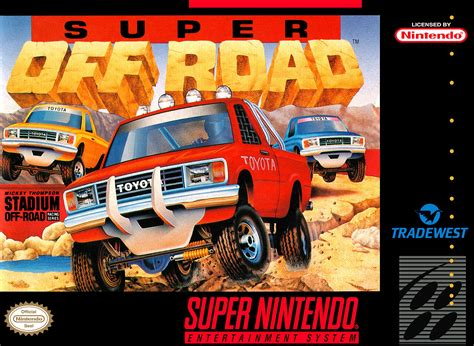
\includegraphics[width=\textwidth]{superOffRoad.jpeg} 
	\end{minipage}
    \vfill
    {\large \@date}
  \end{center}%
  \par
  \vskip 1.5em
  \pagestyle{empty}}
\makeatother

\rmfamily
\renewcommand{\tt}[1]{\texttt{#1}}

\begin{document}

\maketitle

\newcounter{Exercice}
\newcounter{Question}[Exercice]
\newcounter{Lettre}[Question]

\tableofcontents 

\pagebreak

\chapter*{Introduction}

Les jeux analysés dans ce rapport sont Puyo Puyo et Super Off Road. 

Puyo Puyo est un jeu de type puzzle sorti en 1991.

Super Off Road est un jeu de type course sorti en 1989. 


\chapter{Puyo Puyo}

\section*{Introduction}
\addcontentsline{toc}{section}{Introduction}

Puyo puyo est un jeu vidéo de type puzzle développé par Compile. Il est initialement sorti en 1991 sur console, avant que Sega le commercialise en 1992 sur borne d'arcade. Il est devenu le jeu le plus populaire au Japon avant la sortie de Street Fighter 2. 

Le joueur contrôle deux "puyo", deux blocs de couleur aléatoires, qu'il peut faire tourner ou déplacer latéralement. Ces blocs sont soumis à la gravité et s'arrêtent lorsqu'ils reposent sur d'autres blocs. Les puyos se collent entre eux s'ils sont de la même couleur, et 4 puyos adjacents ou plus disparaissent, faisant tomber les puyos au-dessus. 

Il existe aussi un mode duel, où un enchaînement effectué par un joueur ralentit l'adversaire. En effet, plus l'enchaînement est long, plus l'adversaire reçoit des blocs gris encombrants qui ne peuvent être détruits qu'en effectuant des nouvelles combinaisons. 


\section{État du jeu}
\subsection{Structure générale et variables}

La structure générale, ne représentant pas un objet du jeu, est : 
\lstinputlisting[language=pdl]{pdl/puyopuyo/Position.txt}

Cette structure permet d'enregistrer la position d'un objet, que ce soit sur la grille en pixels ou dans la matrice avec i et j. 
\\

Les variables générales sont : 
\begin{itemize}
\item constante entier NBCOLORS 
\item constante entier HEIGHT
\item constante entier WIDTH
\item constante entier FALLSPEED 
\item constante entier SIZEPUYO
\item constante entier WIDTHMAT
\item constante entier HEIGHTMAT
\item constante entier WAITINGPOSX
\item constante entier WAITINGPOSY
\item booleen startTour
\\
\end{itemize}

\begin{itemize}
\item[\textbf{constante entier NBCOLORS}] permet de stocker le nombre de couleurs différentes dans le jeu.
\item[\textbf{constante entier HEIGHT}] détermine la hauteur en pixels du plateau de jeu d’un joueur.
\item[\textbf{constante entier WIDTH}] détermine la largeur en pixels du plateau de jeu d’un joueur.
\item[\textbf{constante entier FALLSPEED}] représente la vitesse à laquelle les Puyo tombent.
\item[\textbf{constante entier SIZEPUYO}] représente la taille en pixels d’un côté d’un puyo.
\item[\textbf{constante entier WIDTHMAT}] représente la longueur des lignes de la matrice de blocs.
\item[\textbf{constante entier HEIGHTMAT}] représente la longueur des colonnes de la matrice de blocs.
\item[\textbf{constante entier WAITINGPOSX}]
\item[\textbf{constante entier WAITINGPOSY}] représentent la position de l'affichage des Puyo en attente. 
\item[\textbf{booleen startTour}] détermine si un tour va commencer ou non. 

\end{itemize}

\subsection{Structure Block}

\lstinputlisting[language=pdl]{pdl/puyopuyo/Block.txt}

Ce type agrégé représente un Puyo, c'est-à-dire un bloc de couleur (variable \tt{color}). Il est stocké dans une matrice \tt{blocks}, qui répertorie la position de chaque bloc. Le booléen \tt{exist} est ici pour savoir si les cases de la matrice sont vides ou non. Afin de connaître les combinaisons de puyos faites sur le jeu, on utilise \tt{groupID} qui attribue un nombre à chaque combinaison. 
\\

\subsection{Structure BlockFall}

\lstinputlisting[language=pdl]{pdl/puyopuyo/BlockFall.txt}

Ce type agrégé représente les 2 Puyo en train de tomber, ceux sur lesquels le joueur peut agir pour changer leur orientation ou leur position sur la grille. Ils possèdent une orientation (\tt{orient}), allant de 0 à 3 (0 pour la gauche, 1 pour le haut, 2 pour la droite et 3 pour le bas). Chaque puyo possède une couleur spécifique (\tt{color1}, \tt{color2} avec comme valeur '\tt{r}','\tt{b}','\tt{g}','\tt{y}' ou '\tt{p}') qui permet de créer des combinaisons de blocs de même couleur. Ils ont également une position (\tt{pos}) sur la grille et une position (\tt{posMat}) dans la matrice de stockage des Puyo. Leur vitesse de chute est déterminée par l'entier \tt{speed}.  
\\

\subsection{Structure Player}

\lstinputlisting[language=pdl]{pdl/puyopuyo/Player.txt}

Le joueur est attaché à une matrice \tt{blocks} dans laquelle sont stockés les Puyo présents sur la grille de jeu. Détruire des combinaisons de Puyo augmentent son \tt{score}. On lui associe aussi un premier BlockFall \tt{bf1} qui est présent sur la grille, et un deuxième BlockFall \tt{bf2} qui est affiché à côté de la grille et qui est le prochain à tomber. 
\\

\subsection{Structure Game}

\lstinputlisting[language=pdl]{pdl/puyopuyo/Game.txt}

Chaque joueur est associé à un jeu (\tt{Game}) de deux joueurs.
\\

\section{Évolution du jeu}

\subsection{Configuration initiale}

\lstinputlisting[language=pdl]{pdl/puyopuyo/startGame.txt}

Le jeu commence avec deux plateaux de jeux vides côte à côte, un pour chaque joueur. La matrice \tt{blocks} de chaque joueur est initialisée avec des blocs vides. Le score des joueurs est à 0, et deux Puyo commencent à tomber sur chaque plateau, en partant du milieu, sur la ligne la plus haute. 

On initialisera aussi un booléen doStartTour à vrai, qui permettra de lancer le premier tour.
\\

\subsection{Règles du jeu}

Le jeu se termine une fois que les nouveaux Puyo ne peuvent plus accéder à la grille d'un joueur, c'est-à-dire quand les deux blocs où ils apparaissent sont déjà occupés par d'autres Puyo qui ne sont pas détruits par combinaisons et lorsque la colonne est remplie d'autres Puyo. Le joueur a alors perdu, et son adversaire gagne. 

\subsection{Actions du joueur}
Le joueur peut effectuer plusieurs actions lors du jeu : il peut déplacer les Puyo en train de tomber sur le côté (on nommera respectivement L et R les touches enfoncées pour déplacer à gauche ou à droite les Puyo), les faire tomber plus vite (touche D) ou changer leur orientation (touches directionnelles). 

Le code 	qui suit est écrit sur la base du joueur 1, on appliquera implicitement ce même code au joueur 2. 

évènement : touche L enfoncée :
\lstinputlisting[language=pdl]{pdl/puyopuyo/leftMotion.txt}

Respectivement, pour la touche R : 
\lstinputlisting[language=pdl]{pdl/puyopuyo/rightMotion.txt}

Ainsi, lorsque le joueur souhaite se déplacer d'un côté, le déplacement sera effectué si le Puyo n'est pas blocké par le bord de la grille de jeu ou par un autre Puyo. 

Évenement : Touche D enfoncée : 
\lstinputlisting[language=pdl]{pdl/puyopuyo/downMotion.txt}

Évenement : Touche D relâchée : 
\lstinputlisting[language=pdl]{pdl/puyopuyo/stopDownMotion.txt}

Lorsque la touche est enfoncée, la vitesse de chute du Puyo est multipliée par 2. Lorsqu'elle est relâchée, elle revient à sa valeur initiale. 

Pour changer l'orientation des Puyo en train de tomber, le joueur appuie sur l'une des quatres touches directionnelles. Si le bloc est vide, et qu'il est dans les limites du jeu, alors le changement de direction se fait. 

Événement : Touche directionelle gauche enfoncée : 
\lstinputlisting[language=pdl]{pdl/puyopuyo/leftOrient.txt}

Événement : Touche directionelle haut enfoncée : 
\lstinputlisting[language=pdl]{pdl/puyopuyo/upOrient.txt}

Événement : Touche directionelle droite enfoncée :
\lstinputlisting[language=pdl]{pdl/puyopuyo/rightOrient.txt}

Événement : Touche directionelle bas enfoncée :
\lstinputlisting[language=pdl]{pdl/puyopuyo/downOrient.txt}

\subsection{Évolutions automatiques de l’état du jeu}

\lstinputlisting[language=pdl]{pdl/puyopuyo/initBlockFall.txt}

L’action initBlockFall permet d’initialiser un tour en reprenant les valeurs du blockFall suivant, au duo de Puyo, notamment les couleurs et la vitesse. Ensuite, on initialise le duo de Puyo en haut de la matrice. 

\lstinputlisting[language=pdl]{pdl/puyopuyo/SwitchColor.txt}

Cette fonction retourne un caractère dépendant de l'entier \tt{nb} envoyé en paramètre d'entrée. Ce caractère représente une couleur de Puyo. 

\lstinputlisting[language=pdl]{pdl/puyopuyo/random0toNb.txt}

Cette fonction retourne un entier aléatoire tiré entre 0 et \tt{nb}. 

\lstinputlisting[language=pdl]{pdl/puyopuyo/randBlockFall.txt}

L’action randBlockFall crée un nouveau BlockFall, avec une orientation égale à 3, c’est-à-dire en bas, deux couleurs aléatoires, initialise sa vitesse, et le positionne à l’emplacement où sera affiché le prochain block qui tombera.

\lstinputlisting[language=pdl]{pdl/puyopuyo/startTour.txt}
La fonction startTour permet d’initialiser un tour. Pour cela, elle fait appel à la fonction initBlockFall pour commencer la descente d'un nouveau duo de Puyos et à la fonction randBlockFall qui crée un nouveau duo de Puyos, indiquant au joueur quel sera le prochain duo. Ensuite, on insère le blockFall dans la matrice, pour la bonne continuation du jeu.

\lstinputlisting[language=pdl]{pdl/puyopuyo/blockTest.txt}

La fonction blockTest retourne un booléen selon l’existence d’un block à l’emplacement indiqué en paramètres d'entrée. Elle retourne vrai s'il n'y a pas de block, faux s'il y en a un. 

\lstinputlisting[language=pdl]{pdl/puyopuyo/doGravityOnAll.txt}

La fonction doGravityOnAll permet de faire agir une pseudo-gravité sur le jeu. Pour cela, le sous-algorithme teste tour à tour chaque colonne de la matrice représentant le jeu. Pour chacune d’elle, on teste la présence d’un bloc grâce au sous-algorithme blockTest. S’il est retourné vrai, c’est-à-dire si le bloc est vide, tous les éléments de la colonne au-dessus de cette ligne sont « descendus » d’un. Ainsi, à la fin de la fonction, tous les blocs se trouvant auparavant au-dessus de vide sont maintenant posés au plus bas.

\lstinputlisting[language=pdl]{pdl/puyopuyo/continueFall.txt} 

La fonction continueFall permet de vérifier si le block en-dessous du duo de Puyo est libre ou non. Il retourne un booléen qui prend la valeur vraie si le block est vide. Pour cela, on doit prendre en compte l'orientation du blockFall.

\lstinputlisting[language=pdl]{pdl/puyopuyo/blockDown.txt}

L'action blockDown insère le deuxième Puyo du duo de Puyo dans la matrice une fois que le duo termine sa chute. 

\lstinputlisting[language=pdl]{pdl/puyopuyo/countNbBlocksEqualID.txt}

La fonction countNbBlocksEqualID permet de retourner la longueur de la chaine auquel appartiennent les blocs possédant un ID égal à l’argument de la fonction.

\lstinputlisting[language=pdl]{pdl/puyopuyo/resetBlocksForID.txt}

Fonction réinitialisant un bloc pour un ID précis donné dans les valeurs d’entrées, via une double boucle permettant de visualiser l’ensemble de la matrice.

\lstinputlisting[language=pdl]{pdl/puyopuyo/destroyBlock.txt}

La fonction destroyBlock permet de détruire l’ensemble des chaînes de 4 Puyo ou plus, via leur ID. Pour cela, on utilise le sous-algorithme countNbBlocksEqualID en testant tous les ID possibles. Ensuite, la fonction réinitialise l’ensemble des ID des Blocks à 0.
De plus, la fonction compte et retourne le nombre de chaines de Puyo supprimées au cours de la fonction.

\lstinputlisting[language=pdl]{pdl/puyopuyo/setClearBlocksOnPlayer.txt}

La fonction setClearBlocksOnPlayer permet d’envoyer des malus au joueur sélectionné dans les paramètres d’entrée. Pour chaque malus envoyé (nombre de répétition reps), la fonction tire une colonne aléatoire, d’où le bloc de malus sera créé. Si un bloc est déjà présent en haut de cette colonne, le bloc de malus n'est pas créé. Cela permet de ne pas trop pénaliser le joueur si sa grille est déjà très remplie.  

\lstinputlisting[language=pdl]{pdl/puyopuyo/blockAtStart.txt}

\lstinputlisting[language=pdl]{pdl/puyopuyo/AttribuerGroupe.txt}

Ici, nous avons un algorithme qui prend en arguments un tableau représentant le jeu du joueur (\tt{Matrice}), la position \tt{posBlock} du block dont on va tester l'appartenance à une chaîne et l'ID de la chaîne (\tt{groupID}). En paramètres de sortie, on aura la matrice avec, pour chaque block, l'ID de la chaîne auquel il appartient ainsi que la longueur de cette chaîne (avec l'ID donné en paramètre). On pourra noter que, s'il n'existe pas de chaîne pour le block à la position \tt{pos}, il ne prendra pas l'ID passé en argument et gardera donc son ID initial. 

Pour le bon fonctionnement de cet algorithme, il faut, avant de le lancer, réinitialiser les ID de tous les blocks à 0 afin que les chaînes soient comptabilisées correctement.

Encore une fois, l'algorithme s'applique au joueur 1 et s'appliquera implicitement au joueur 2 dans cette boucle principale. 
\lstinputlisting[language=pdl]{pdl/puyopuyo/boucleJeu.txt}

Ainsi, la boucle principale commence par lancer un nouveau tour. Un nouveau duo de Puyo commence à tomber avec la fonction \tt{doGravityOnAll}, et les actions du joueur peuvent modifier sa trajectoire.  
Une fois qu'il se pose sur un Puyo ou au sol (vérifié par la fonction \tt{continueFall}), on regarde s'il a effectué une ou plusieurs combinaisons de 4 Puyo ou plus avec \tt{checkAllChains}. Cela permet ensuite de compter puis détruire ces combinaisons (\tt{destroyBlock}). Selon le nombre de combinaisons effectuées, on incrémente la pénalité de l'autre joueur. On ajoute aussi la pénalité qui a été donnée par l'autre joueur. Enfin, on vérifie que le bloc d'arrivée du duo de Puyo est vide (\tt{blockAtStart}), sans quoi le jeu se termine. Une fonction \tt{gameOver} sera implémentée à la fin de la boucle pour traiter la fin du jeu. 








































\chapter{Super Off Road}

\section*{Introduction}
\addcontentsline{toc}{section}{Introduction}

Super off road est un jeu vidéo de type course développé par Leland Corporation. Il est sorti en 1989 sur borne d'arcade avant d'être adapté sur diverses consoles et ordinateurs. 

Le joueur contrôle un monster truck et doit avancer plus vite que ses 3 concurrents, sur un terrain accidenté qui présente bosses, trous, eau, barrières, montées et descentes qui font accélérer ou ralentir le véhicule. En gagnant, il récupère de l'argent qu'il peut utiliser pour modifier et améliorer son véhicule. 

\section{État du jeu}
\subsection{Structures générales et variables}

Les structures générales, ne représentant pas des objets du jeu, sont : 

\subsubsection{Structure Hitbox2P}

\lstinputlisting[language=pdl]{pdl/superOffRoad/Hitbox2P.txt}
La structure \tt{Hitbox2P} permet de stocker deux coordonnées dans le plan, cela afin de former une hitbox en forme de ligne, notamment utile pour les murs ainsi que pour les flags. 

\subsubsection{Structure Hitbox4P}

\lstinputlisting[language=pdl]{pdl/superOffRoad/Hitbox4P.txt}
La structure \tt{Hitbox4P} est la même que la structure \tt{Hitbox2P} sauf qu'elle permet de stocker 4 coordonnées et non pas 2, cela afin de former une hitbox en forme de quadrilatère notamment en forcorrigéme de rectangle pour la voiture ou en forme de carré pour les bonus. Les types corner1,2,3 et 4 représente donc les sommets de ce quadrilatère.


\subsubsection{Structure Position}

\lstinputlisting[language=pdl]{pdl/superOffRoad/Position.txt}
La structure \tt{Position} permet de stocker les coordonnées d'un point dans le plan, l'entier \tt{x} étant la coordonnée en x et \tt{y} la coordonnée en y.

\subsubsection{Structure Speed}

\lstinputlisting[language=pdl]{pdl/superOffRoad/Speed.txt}




Les variables générales sont : 

\begin{itemize}
  \item constante entier ACCELERATION
  \item constante entier NB\_LAPS
  \item constante entier MIN\_TIME\_DROP\_NITRO
  \item constante entier MAX\_TIME\_DROP\_NITRO
  \item constante entier NITRO\_TIME
  \item constante entier NITRO\_WIDTH
  \item constante entier NITRO\_SPAWN\_TIME
  \item constante entier CAR\_WIDTH
  \item constante entier CAR\_HEIGHT
  \item Car playerCar
  \item Bonus [] nitroList
  \item entier malusBonusSpeed <- 1
  \\
\end{itemize}

\begin{itemize}
  \item [\textbf{constante entier ACCELERATION}]permet de stocker l'accélération de la voiture lorsque le joueur avance.
  \item [\textbf{constante entier NB\_LAPS}]permet de stocker le nombre de tour demandé pour finir la course et gagner la partie.
  \item[\textbf{constante entier NITRO\_TIME}]permet de stocker le temps durant lequel le boost de vitesse donné par la nitro est actif.
  \item[\textbf{constant entier NITRO\_WIDTH}]Stocke la longueur d'un côté de la hitbox du bonus de nitro.
  \item[\textbf{comstante entier NITRO\_SPAWN\_TIME}]Stocke le temps entre chaque génération d'un bonus de nitro sur la carte.
  \item[\textbf{constante entier CAR\_WIDTH}]Permet de stocké la longueur de la hitbox de la voiture.
  \item[\textbf{constant entier CAR\_HEIGHT}]Perment de stocké la largeur de la hitbox de la voiture.
  \item[\textbf{Car playerCar}]Cette variable de type \tt{Car} va stocker toute les information relative à la voiture du joueur.
  \item[\textbf{Bonus [] nitroList}]Ce tableau de variable de type \tt{Bonus} permet de stocker les information relative a l'emplacement des bonus de nitro présent sur la map.
  \item[\textbf{entier malusBonusSpeed <- 1}]Cette entier stocke un multiplicateur de l'accélération ce qui perment d'influencer sur la vitesse de la voiture lorsque celle-ci rencontre un mur ou de la boue.
\end{itemize}

\subsection{Structure Flag}


\lstinputlisting[language=pdl]{pdl/superOffRoad/Flag.txt}
Les flags sont des lignes invisibles que le joueur traversera afin de vérifier qu'il fait bien la course dans le bon sens et qu'il ne se retourne pas juste pour franchir trois fois d'affiler la ligne d'arrivé. le type structuré hitbox2P contient les deux coordonnées qui délimite les extrémités du segment qu'est la hitbox et la position du flag. le type nb contient la position du flag sur le trajet du joueur (0 pour la ligne de départ et d'arrivé, 1 pour le premier flag censé etre traversé par le joueur,etc ...).

\subsection{Structure Wall}

\lstinputlisting[language=pdl]{pdl/superOffRoad/Wall.txt}
Les wall sont les éléments du décors qui délimite les bordures du circuits de course, dans ce type structuré, on y trouve le type structuré hitbox2P qui permet de stocké les deux points qui forment les extrémités de la ligne qui forme la hitbox du mur ainsi que sa position. Nous trouvons aussi l'entier \tt{directionStop} qui stocke la direction dans laquel la voiture du joueur doit arrivé pour etre stoppé nette et pas redirigé (cette direction est colinéaire la normal de la ligne qui forme la hitbox du mur).

\subsection{Structure Car}

\lstinputlisting[language=pdl]{pdl/superOffRoad/Car.txt}


\subsection{Structure Bonus}

\lstinputlisting[language=pdl]{pdl/superOffRoad/Bonus.txt}
La structure \tt{Bonus} permet de stocker les informations de position d'un bonus, aavec le type \tt{pos} ainsi que sa hitbox avec le type \tt{hitbox}.

\subsection{Structure Mud}

\lstinputlisting[language=pdl]{pdl/superOffRoad/Mud.txt}
La structure \tt{Mud} permet de stocker la position d'un obstacle de boue, avec le type \tt{pos} et sa hitbox, avec le type \tt{hitbox}.


\section{Évolution du jeu}

\subsection{Configuration initiale}

\lstinputlisting[language=pdl]{pdl/superOffRoad/InitialisationProgram.txt}
Dans la phase d'initialisation du jeu il y a d'abord la déclaration de plusieurs variable très utile, le réel \tt{timer} qui permetera de ne faire aparaitre un bonus a un certain intervalle de temps. 

La variable \tt{level} de type \tt{ground} qui va stocker les listes de touts les objets important du jeu, la liste de tout les murs (\tt{level.walls}) (Cette liste sera remplie à la main pour que les hitboxs et positions des murs corespondent avec le background.), la liste de tout les flags (\tt{level.flags}), la encore cette liste sera remplie à la main pour correspondre avec le circuit, idem pour la liste \tt{level.muds} et pour la liste \tt{level.spawnPosNItro} qui elle contient les emplacements possible de l'apparition des bonus de nitro.

La variable \tt{playerCar}, de type \tt{Car} qui stockera les informations contenant la voiture du joueur, sa position en x et en y sera rentré a la main pour correspondre avec la ligne de départ du circuit, sa vitesse (\tt{playerCar.Speed}) est initialisé a 0, pareil pour le nombre de tour effectué (\tt{playerCar.laps}) et le nombre de flag franchie (\tt{playerCar.flag}).
Le nombre de nitro disponible au début de la course est fixé à 3 (\tt{playerCar.nbNitro}).

Les booléens \tt{haut}, \tt{bas}, \tt{gauche}, \tt{droite}, et \tt{nitro} sont des variables qui vont stocker les action effectuer par le joueur lorsqu'il appuis sur les touches pour après pouvoir modifier l'état du jeu, par défaut, ces variables sont initialisées à faux.

Voila pour l'initialisation du jeu.

\subsection{Règles du jeu}

Super off road est un jeu de course de voiture dont le but est d'être le premier à compléter 3 tours d'un circuit en terre avec des obstacles tels que des bosses, des montées et descentes, des flaques de boue et autres. Le circuit est délimité par des palissades infranchissables. Pour être le premier, le joueur dispose avant le début de la course d'une certaine quantité d'argent qu'il peut utiliser pour s'acheter des améliorations comme un moteur plus puissant, des roues plus adhérentes ou encore de la nitro utilisable pendant la course pour s'octroyer un boost de vitesse temporaire.

\lstinputlisting[language=pdl]{pdl/superOffRoad/ReglesDuJeuMurs.txt}

Pendant la boucle on va d'abord tester si la voiture a rencontré un mur. On va donc tester avec la fonction iscollision 
\subsection{Actions du joueur}


\lstinputlisting[language=pdl]{pdl/superOffRoad/ActionDuJoueur.txt}

Les actions que le joueur peut effectuer sont les suivante, il peut apuyer sur la touche z, ce qui mettra le booléen \tt{haut} à vrai jusqu'a ce qu'il la relache, cela à pour effet de faire accélérer la voiture, il peut appuyer sur la touche q ce qui mettra le booléen \tt{gauche} à vrai (toujours juqu'a ce qu'il la relache) ce qui aurra pour effet d'incrémenter la variable \tt{playerCar.direction} de -1 ce qui fera tourner la voiture vers la gauche.
Il peut appuyer sur la touche s ce qui mettra la variable \tt{bas} à vrai ce qui fera freiner la voiture. Il peut appuyer sur la touche d, ce qui mettra la variable \tt{droite} à vrai ce qui incrémentera la direction de 1 et fera tourner la voiture vers la gauche.
Et enfin, il peut appuyer sur la barre espace ce qui mettra la variable \tt{nitro} à vrai et donc consomera une charge de nitro pour accorder un boost de vitesse temporaire.

\subsection{Alghoritmes}

\subsubsection{title}

\lstinputlisting[language=pdl]{pdl/superOffRoad/calculateNorme.txt}

Cette fonction calcule la norme d'un vecteur à partir de sa longueur en \tt{x} et en \tt{y}.

\subsubsection{title}

\lstinputlisting[language=pdl]{pdl/superOffRoad/calculateSpeed.txt}

Cette fonction prend en paramètre la voiture dont on veux calculer la vitesse (\tt{car}), l'accéleration de cette voiture (\tt{acceleration} ainsi que l'accélération standard (\tt{avgAcceleration}) et le temps depuis la dernière itération (\tt{dt}). On renvoie la nouvelle vitesse de la voiture grâce à la structure \tt{speed}. On peut changer la vitesse selon différentes conditions du jeu. En utilisant un boost, elle augmente, si la voiture est dans la boue, elle diminue. Enfin, si le joueur n'effectue aucune action, l'accélération tombe à 0.

\subsubsection{title}

\lstinputlisting[language=pdl]{pdl/superOffRoad/moveCar.txt}

Cette fonction simple modifie la position de la voiture en fonction du temps écoulé depuis la dernière itération (\tt{dt}).


\subsubsection{getAxisList}

\lstinputlisting[language=pdl]{pdl/superOffRoad/getAxisList.txt}

Cette fonction prend en entrer un tableau de point dans le plans et calcul pour chaque arretes du polygone convexe formé par cette ensemble de point le vecteur unitaire normal à la droite formé par l'arrete.
cette alghoritme retourne donc une liste de vecteur unitaire, tous normal à une arrete du polygone formé par la liste de point.

\subsubsection{getProject}


\lstinputlisting[language=pdl]{pdl/superOffRoad/getProject.txt}

Cette


\subsubsection{title}

\lstinputlisting[language=pdl]{pdl/superOffRoad/isColisionAxis.txt}

\subsubsection{title}

\lstinputlisting[language=pdl]{pdl/superOffRoad/isColision.txt}

\subsubsection{title}

\lstinputlisting[language=pdl]{pdl/superOffRoad/ToList.txt}

\subsubsection{title}

\lstinputlisting[language=pdl]{pdl/superOffRoad/calculDeLaHitbox.txt}

\subsubsection{title}

\lstinputlisting[language=pdl]{pdl/superOffRoad/countTour.txt}


\chapter*{Conclusion}

\addcontentsline{toc}{chapter}{Conclusion}

\begin{abstract}
Résumé / Abstract
\end{abstract}

\end{document}
